%%%--------------------------------%%%
%%% UC6
%%%--------------------------------%%%

\newpage
% UC6 ====================================================
\subsubsection{Use Case Specification: \ac{UC}6 Risk Discussion}
\label{sec:domainBbg}
\paragraph*{Description}\mbox{}\\
The process of adding risks to a project is based on three steps:
\begin{enumerate}
	\vspace{-3mm}
	\setlength\itemsep{-1em}
	
	\item A project member proposes a risk (name and description). (UC3 Risk CRUD defined in chapter \ref{sec:domainBbd}).
	\item A specified number of project members review the proposed risk. After the review process the risk is ready for discussion.
	\item The whole project team discusses and defines:
	\begin{itemize}
		\vspace{-3mm}
		\setlength\itemsep{-1em}
		
		\item probability of occurence
		\item impact
		\item risk factor (defined by probability of occurence and impact)
		\item response(s)
		\item person in charge
	\end{itemize}
\end{enumerate}

\begin{figure}[H]
	\centering
	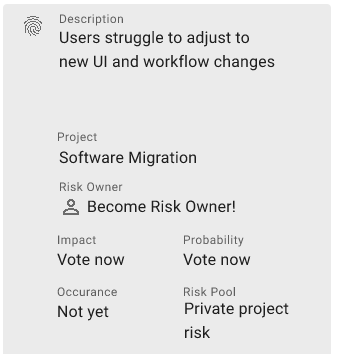
\includegraphics[width=0.3\textwidth]{Assets/UC_Screenshots/UC6S.png}
	\caption{Use Case 6: Mock Prototype}
	\label{fig:useCase6Detail}
\end{figure}

\paragraph*{Basic Flow} \mbox{}\\

\begin{enumerate}
	\vspace{-3mm}
	\setlength\itemsep{-1em}
	
	\item A project member proposes a risk (name and description as defined in UC3 Risk CRUD chapter \ref{sec:domainBbd})
	\begin{itemize}
		\vspace{-3mm}
		\setlength\itemsep{-1em}
		
		\item The proposed risk is visible in the section proposed risks at the project overview page ("Proposed risks").
		\item All members of the project receive a notification (in their activity stream) about the new proposed risk and the request to review it.
	\end{itemize}
	
	\item A specified number of project members review the proposed risk. After the review process the risk is ready for discussion.
	\begin{itemize}
		\vspace{-3mm}
		\setlength\itemsep{-1em}
		
		\item When the specified number of project members have positively reviewed the risk, it is visible in the section ("Risks open to discussion").
		\item The project owner is able to manually start an estimation session for the risk (not recommended). The recommended way is to wait until a specified number of risks open for estimation are collected. Then an estimation session for all risks is automatically started.
	\end{itemize}
	
	\item The risk is estimated by the whole project team:
	\begin{itemize}
		\vspace{-3mm}
		\setlength\itemsep{-1em}
		
		\item All project members receive a notification (in their activity stream) to estimate the risk in terms of (probability of occurrence, impact) and to add response(s). Probability of occurrence and impact are mandatory fields, response(s) are optional.
		\item The risk factor is determined by the probability of occurrence and the impact.
		\item It is checked if at least one response is defined. If not the project members are notified to add a response.
		\item In the last step the person in charge is defined. Therefore a notification where the user is able to sign up for being responsible for the risk is sent to all project members.  
	\end{itemize}
	
	\item Finally the risk appears at the project risk table ("Project risks").
\end{enumerate}

\newpage
\subparagraph{Activity Diagram}\mbox{}\\
\begin{figure}[H]
	\centering
	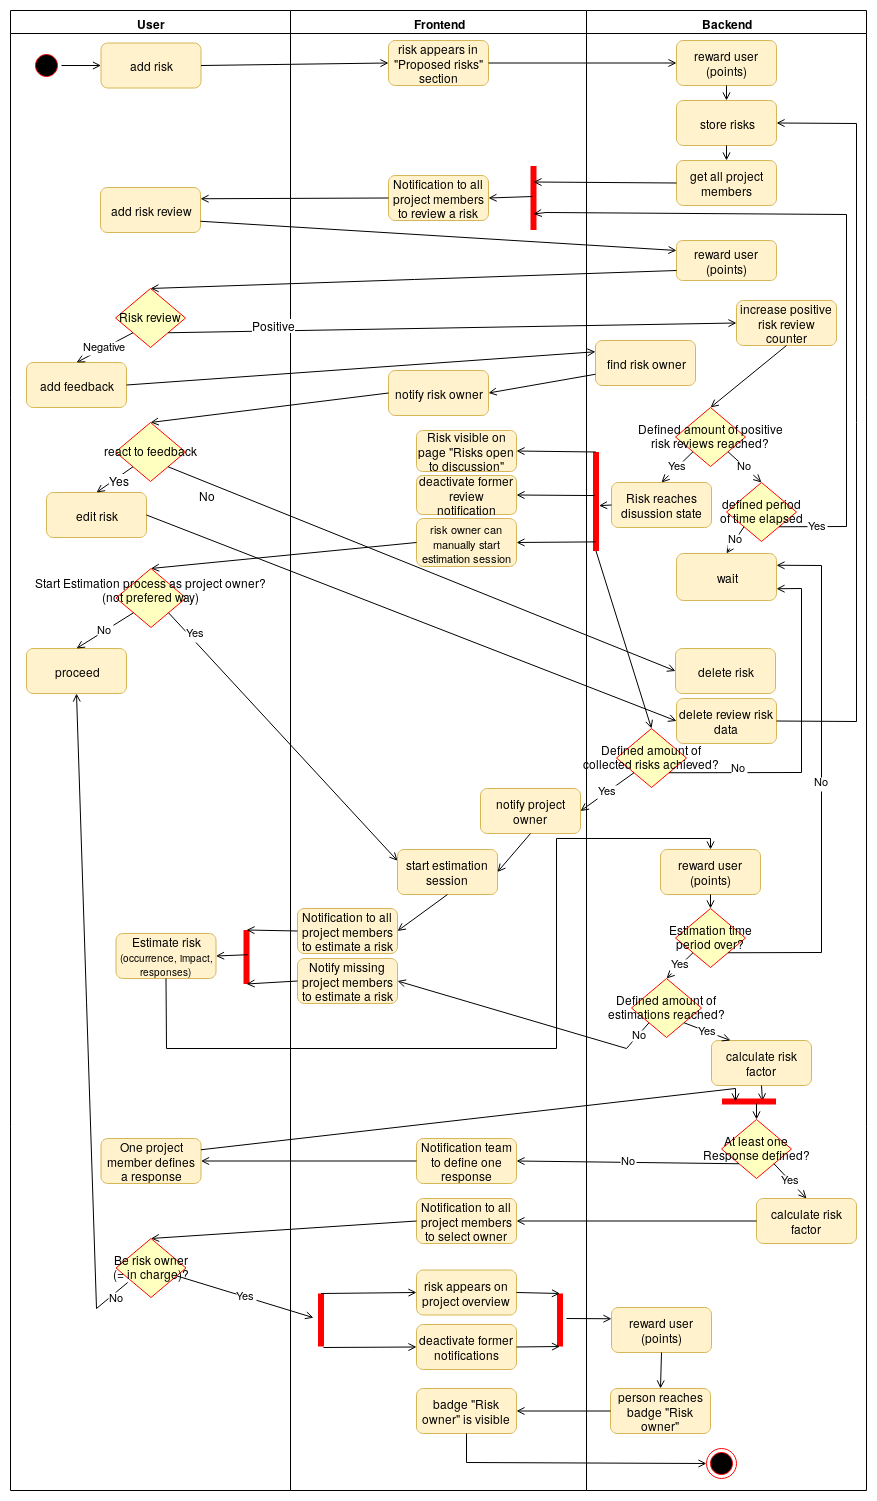
\includegraphics[width=0.70\textwidth]{Content/Domain/UC6RiskDiscussion.png}
	\caption{Activity Diagram \ac{UC}6 Risk Discussion}
	\label{fig:label66}
\end{figure}

\newpage

\paragraph*{Alternative Flows}\mbox{}\\

\noindent
Proposed risk receives negative reviews:
\begin{itemize}
	\vspace{-3mm}
	\setlength\itemsep{-1em}
	
	\item A project member negatively reviews a risk.
	\item The reviewing person adds feedback for the risk which is sent to the risk owner.
	\item The risk owner can edit or delete the proposed risk.
	\item When the risk is deleted it is removed from the section proposed risks.
	\item When the risk is edited the review process data is removed and the message for reviewing is sent again.
\end{itemize}

\noindent
Project members doesn't react to their notifications to:
\begin{enumerate}
	\vspace{-3mm}
	\setlength\itemsep{-1em}
	
	\item review a risk: When the needed amount of reviews is not achieved the notification is sent again.
	\item estimate a risk: When the needed amount of estimations is not achieved the notification is sent again.
	\item define a person in charge: When no person volunteers the notification is sent again. For finding a risk person in charge fast the Gamification concept Challenge is used.
\end{enumerate}

\paragraph*{Special Requirements and Preconditions}\mbox{}\\
The preconditions for this use case are:
\begin{enumerate}
	\vspace{-3mm}
	\setlength\itemsep{-1em}
	
	\item  A project exists.
	\item The user is member of the project.
	\item The user has proposed a risk.
\end{enumerate}

\paragraph*{Postconditions and Persistance}\mbox{}\\
The postconditions for this use case are:
\begin{enumerate}
	\vspace{-3mm}
	\setlength\itemsep{-1em}
	
	\item The proposed risk was reviewed and estimated. 
	\item The risk contains all relevant data.
	\item The risk is visible as part of the projects risk table.
\end{enumerate}

